\chapter{India's struggle for independence: 1857-1947}

\section*{Introduction}
\begin{itemize}
    \item Book Citation : \cite{Bipan__2016}.
    \item India's struggle for independence was unique in its non-violent nature, the robust internal democracy within the Congress movement (as it was called before indepedence), its commitment to secularism and a strongly anti-imperialist foreign policy.
    \item Cambridge School of historians (imperialist) deny fundamentally the existence of colonialism in British India and the contracdiction of between the interests of the Indian subjects and their British rulers.
    \item This school believes that caste, religion and region-based politics are the reality and that any nationalist sentiment is a mere cover.
    \item It also refuses to believe that all the lives sacrificed in the freedom movement were motivated by any idealism.
    \item Nationalist school of \gls{histriography} completely ignores the class, caste and ideological struggles for hegemony within the national freedom movement.
    \item Marxist School, which believes that the movement was led by and belonged to the bourgeoisie primarily, and ignores the all-class nature of the struggle.
    \item A clear anti-colonial ideology and a critique of colonialism evolved at the very beginning of the freedom movement among the Indian intelligentsia.
    \item The making of a national identity was never considered at odds with the religious, regional, linguistic and cultural diversity of the Indian colony.
    \item British rule was not benevolent and not invincible. These were the primary ideas which needed to be disseminated to break the British cultural hegemony within the subcontinent.
    \item Communalist forces did not get eradicated completely by the national movement. Also it could not bring about a full cultural revolution in terms of advancing the social status of women, Harijans, the landless poor and other disadvantaged groups.
    \item Hegemony is means the way a ruling class organizes consent among the ruled and exercised moral authority over them. It does not refer to direct use of force in order to express dominance.
\end{itemize}

\section{The First Major Challenge: The Revolt of 1857}

\begin{itemize}
    \item Bahadur Shah II was coerced into declaring himself the face of the Sepoy Mutiny of 1857, which started in Meerut and marched to Delhi
    \item Since the revolt lacked any organized leadership, local aristocrats and princelings were often the impromptu administrators and leaders of the insurgency
    \item Serving in the British Army conflicted with the sepoys' caste and religious sentiments, especially when deploying overseas
    \item In most places, civil rebellion accompanied the sepoys' mutiny with violent destruction of government property
    \item Increasing economic oppression and draconian land revenue policies also played a role in angering the soldiers
    \item Indian traders, intelligentsia, and royalty did not support the rebels, and sometimes actively supported the \Gls{raj}
\end{itemize}

\begin{marginfigure}[-5.5in]
    \centering
    \framebox{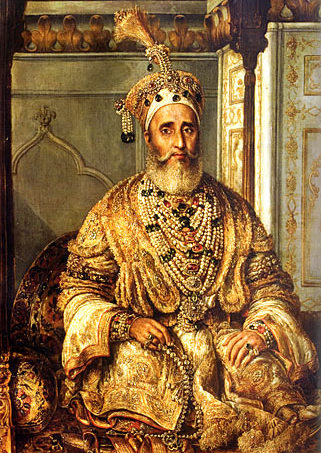
\includegraphics[width=0.75\marginparwidth]{./pictures/Bahadur_Shah_II.jpg}}
    \caption{Bahadur Shah Zafar I}
    \vspace{0.8in}
    \framebox{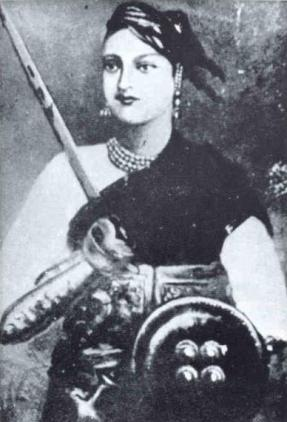
\includegraphics[width=0.75\marginparwidth]{./pictures/Rani_of_Jhansi.jpg}}
    \caption{Rani Lakshmibai of Jhansi}
    \vspace{0.8in}
    \framebox{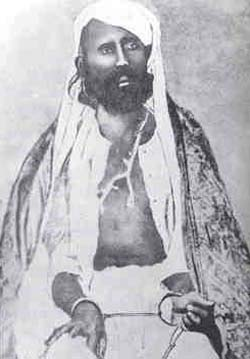
\includegraphics[width=0.75\marginparwidth]{./pictures/Tantiatope.jpg}}
    \caption{Tantia Tope}
\end{marginfigure}

\section{Civil Rebellions and Tribal Uprisings}
\begin{itemize}
    \item Deposed kings and minor princelings often led peasant rebellions in the first 100 years of the Raj
    \item Much greater pressure on the peasants due to increased land revenue collection by the British compared to the Mughals led to discontent
    \item Every class in society lost either their wealth, livelihood, patronage or political power with the advent of the Raj in the late 18th century
    \item These early rebellions were fuelled by local causes and confined to a small geographical spread, completely isolated from each other
    \item Tribals were brought fully into the colonial land-revenue system and denied their semi-isolated lifestyle dependent on the forest for food, cattle-feed and fuel
    \item They were entrapped in debt and unpaid agricultural labor contracts as a result of colonization
    \item Santhal rebellion near Bhagalpur, Kol rebellion in Chhotanagpur, and the Munda rebellion led by Birsa Munda were the three biggest tribal uprisings
    \item Tribal leaders would often proclaim to have received a commandment from God to raise arms against the oppressive outsiders which would be a powerful rallying cry to motivate their tribesmen
\end{itemize}

\begin{marginfigure}[-2in]
    \centering
    \framebox{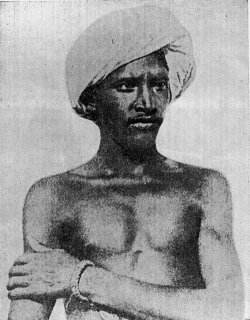
\includegraphics[width=0.75\marginparwidth]{./pictures/Birsa_Munda.jpg}}
    \caption{Birsa Munda}
    \vspace{0.8in}
    \framebox{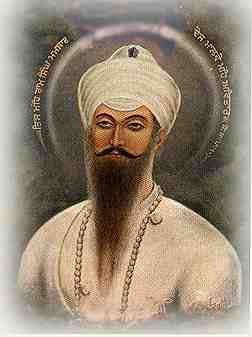
\includegraphics[width=0.75\marginparwidth]{./pictures/Namdhari_Guru_Ram_Singh.jpg}}
    \caption{Guru Ram Singh Kuka}
    \vspace{0.8in}
    \framebox{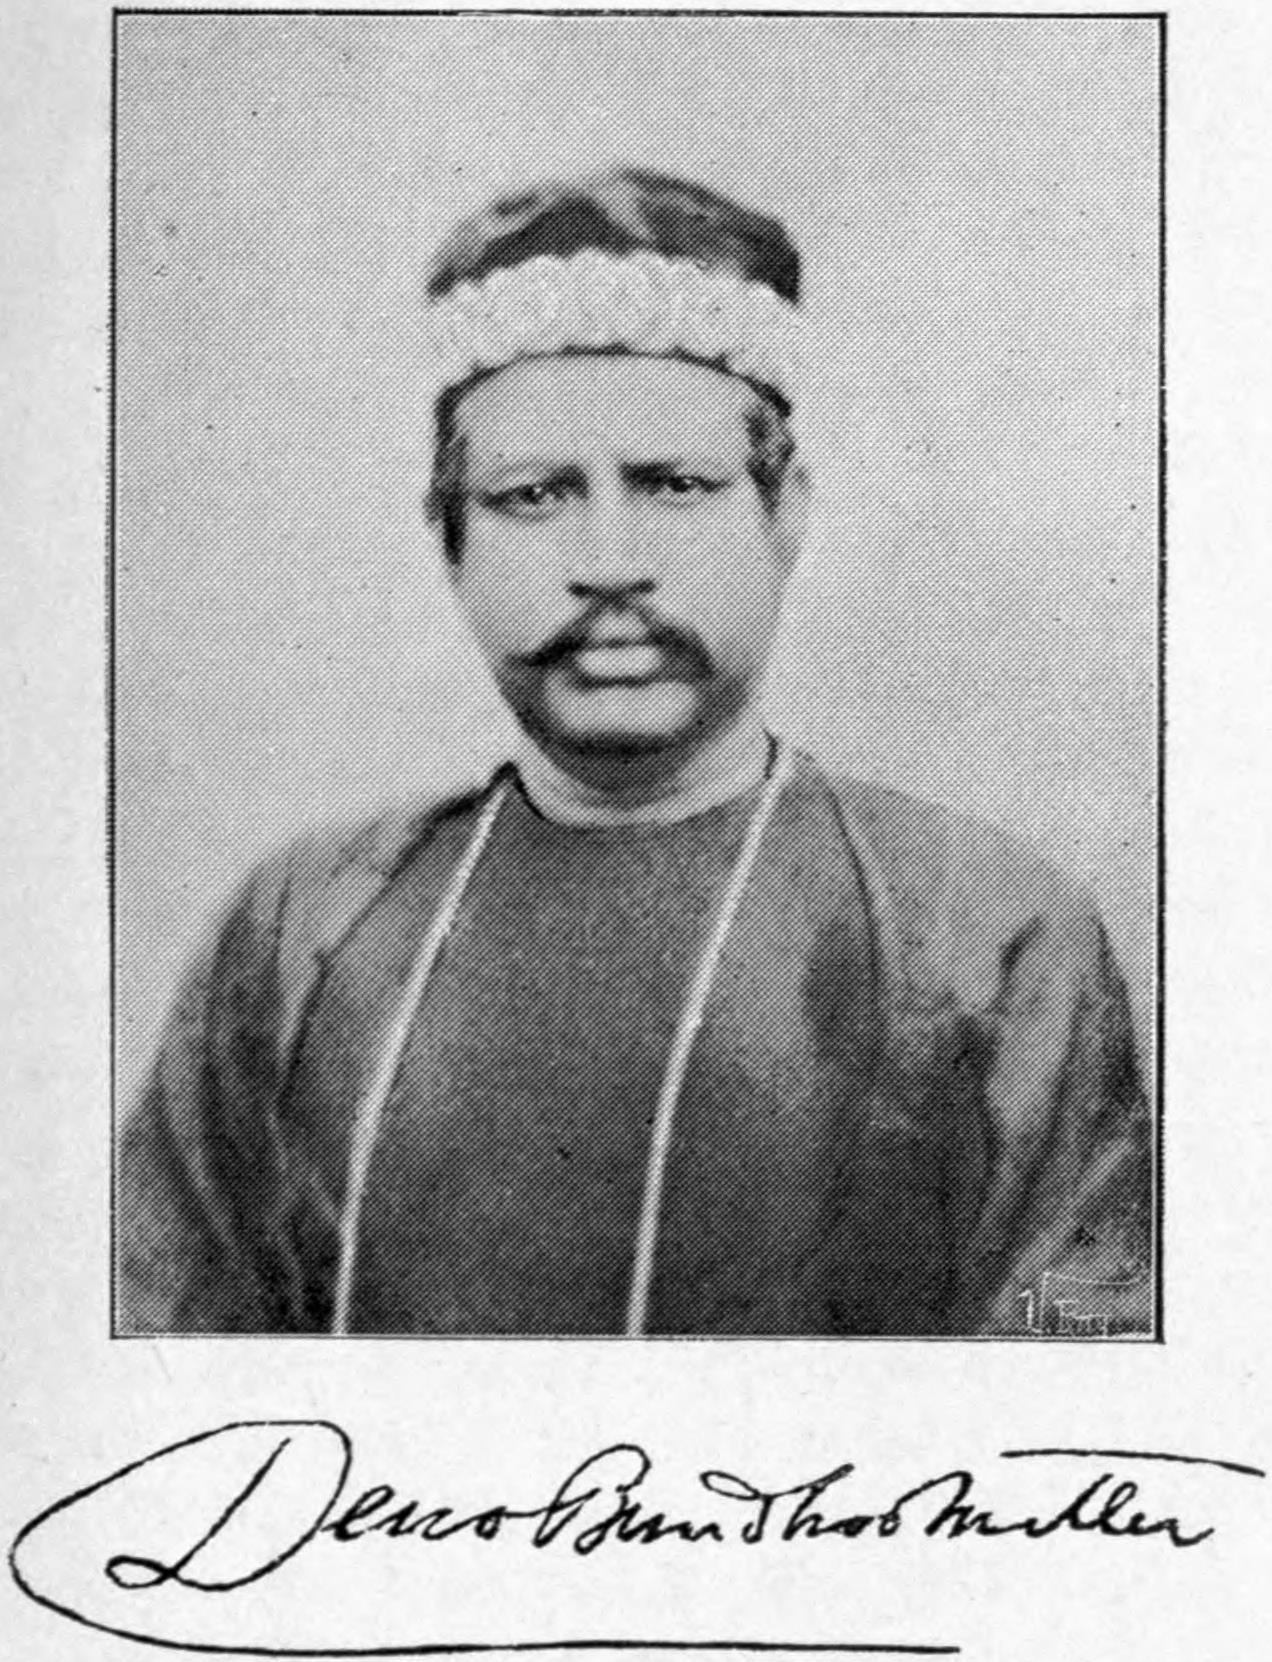
\includegraphics[width=0.75\marginparwidth]{./pictures/Dinobandhu_Mitra.jpg}}
    \caption{Dinabandhu Mitra}
\end{marginfigure}

\section{Peasant Movements and Uprisings after 1857}
\begin{itemize}
    \item Indigo planters in Bengal province forced fraudulent contracts on their peasants, often offering them less than fair prices. They also resrted to the use of brute force to compel the peasants to accept these unfavourable working conditions
    \item Indigo cultivation was successfully wiped out from Bengal by 1860 through the peasants' use of legal resistance, armed insurrection and social boycott
    \item Intelligentsia played a key role in the Indigo protests by collecting and disseminating information about the state of the rebellion throughout the province using the printing press
    \item In legal disputed between the peasants and the \glspl{zamindar}, the Raj took a neutral stance, with help being given to the landowners only on the rare occasion when violence broke out
    \item Cotton farmers in Maharashtra also revolted against the moneylenders and landowners
    \item Peasant revolts in the 1870s were also prevalent in the Malabar and in Punjab and Assam
    \item After 1857, the revolts started to ignore local princes and leaders in favour of being organized entirely by peasants
    \item These protests sought to bring back the old world order, and get rid of the excessive pressure on their land revenue from the British Raj. They did not seek to establish a new world order, or to  upend the existing social hierarchy
    \item Peasant movements were not anti-imperialist and had no issue with the colonial power structure itself. They were merely protesting against the unjust revenue collection and illegal behaviour of their landowners
\end{itemize}


\section{Foundation of the Congress: The Myth}

\begin{marginfigure}[-0.25in]
    \centering
    \framebox{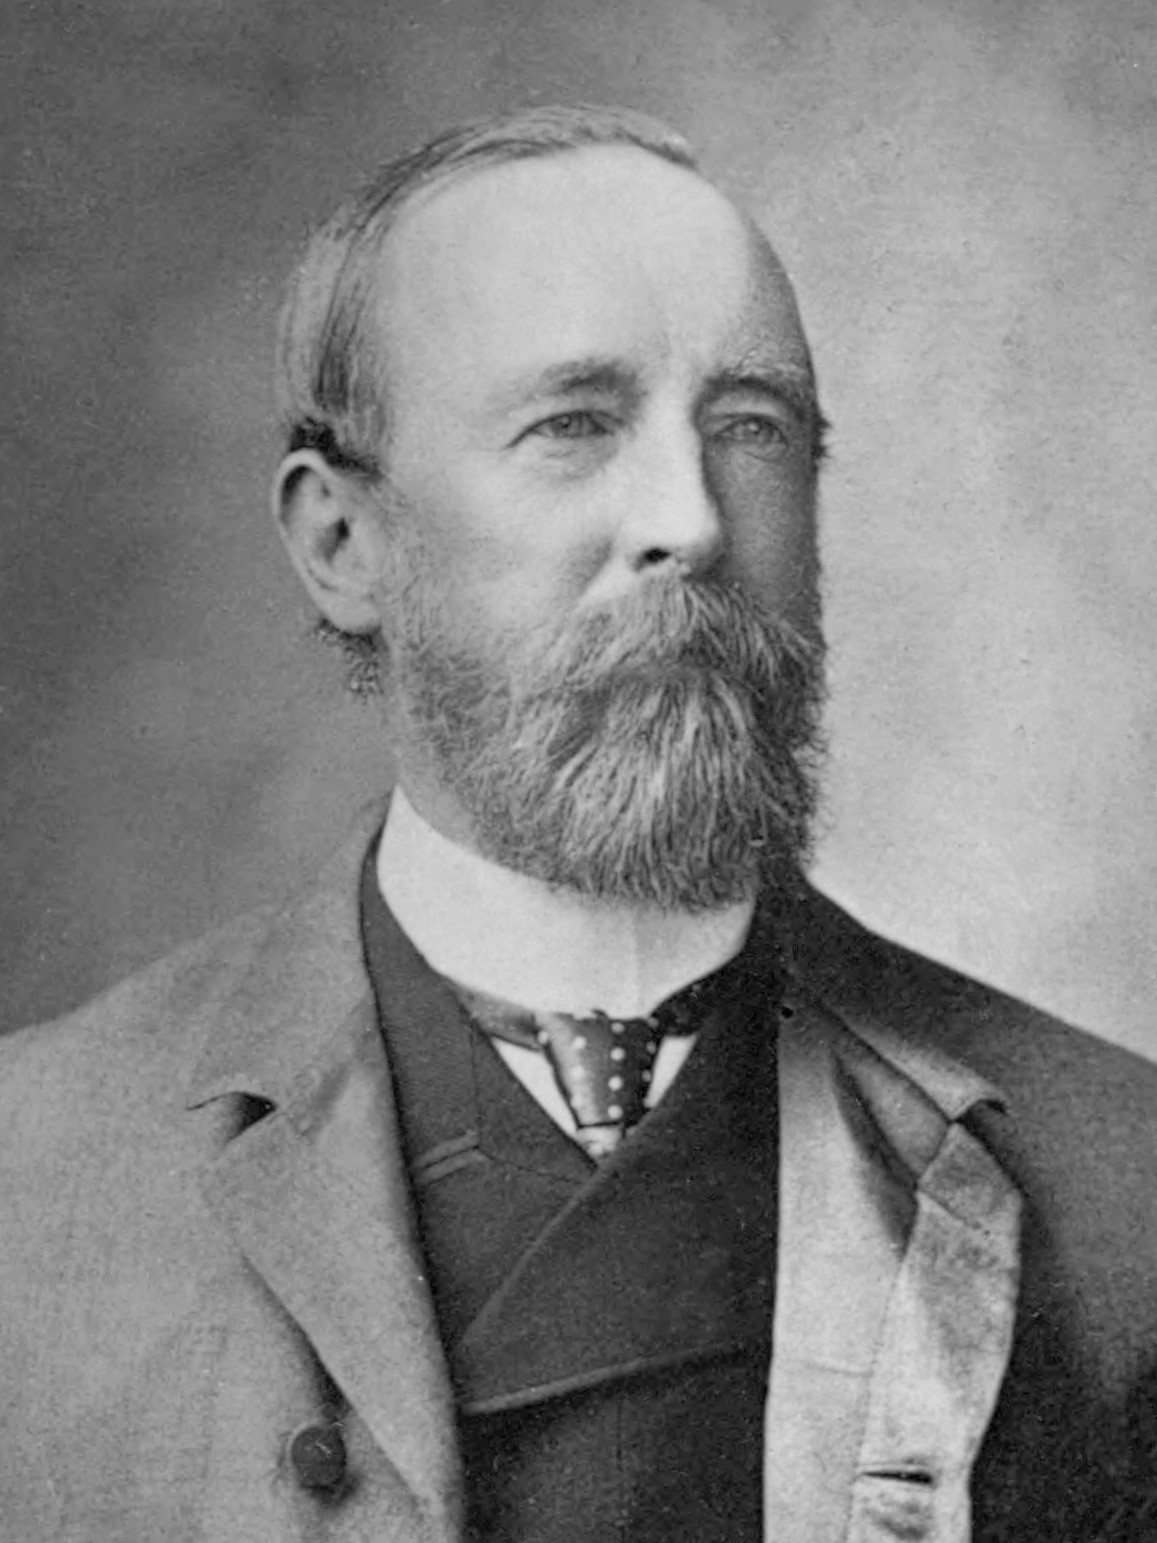
\includegraphics[width=0.75\marginparwidth]{./pictures/A_O_Hume.jpg}}
    \caption{Alexander Hume}
    \vspace{0.8in}
    \framebox{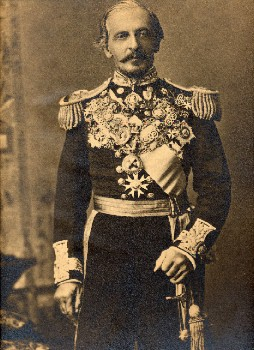
\includegraphics[width=0.75\marginparwidth]{./pictures/Viceroy_Dufferin.jpg}}
    \caption{Viceroy Lord Dufferin}
    \vspace{0.8in}
    \framebox{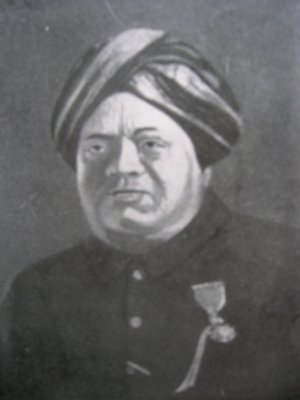
\includegraphics[width=0.75\marginparwidth]{./pictures/Ananda_Charlu.jpg}}
    \caption{P. Ananda Charlu}
\end{marginfigure}

\begin{itemize}
    \item An extremely prevalent myth is that the \gls{inc} was founded in 1885 as a safety valve for the  rising anger under the full supervision and approval of the Raj
    \item The extreme left and extreme right found it convenient to use this myth to attack the non-violence and the secularism of the INC respectively
    \item A.O.Hume, the source of this myth, had corresponded with the Viceroys of the time, talking about his interactions with omniscieent godmen residing in Tibet and their role in quelling the earlier rebellions in India
    \item Extensive written records of communication between Viceroy Dufferin, the Governor of Bombay and A.O.Hume prove that the INC was birthed as a political body and that the Raj did not approve of its existence in the slightest
\end{itemize}

\section{Foundation of The Indian National Congress: The Reality}
\begin{itemize}
    \item Indians had been making less extrmeme demands for financial relief, military and administrative reform and the election of more sympathetic leaders in British elections even before 1885, when the INC was formally founded
    \item Promoting national unity and the idea of India as a nation within the popular consciousness was a major INC objective
    \item Politics of popular participation and mobilization was completely new to India, which had only lived under monarchy for many centuries
    \item Even though the early INC leaders did not organize any mass movements, their role in understanding the nature and purpose of the colonial system and the evolution of a pan-Indian national identity is still a valued contribution to winning India's freedom
    \item A leadership group  or headquarters for the national movement was also necessary. This role was to be fulfilled by the INC using its parlimentary system of decision making during regular sessions held all over the country
    \item Suppression of the INC in its early days was sidestepped by having a distinguished retired \gls{ics} man (A.O. Hume) be the chief organizer
\end{itemize}

\section{Socio-Religious Reforms and the National Awakening}
\begin{itemize}
    \item Political action required social reform which in turn required religious reform, if only from the utilitarian point of view of making the Indian masses more capable of mass political action
    \item Religious reformers of the time were motivated by rationalism and a rejection of the immutability of religious scripture
    \item Priests had a monopoly on communing with the Gods, and on dictating almost every aspect of a layman's life. The reformers sought to break this straglehold and democratize the practise of religion
    \item Reformers also sought to use the natural instinct to oppose the imposition of colonial cultural values towards the awakening of a greater political consciousness among the people
\end{itemize}

\begin{marginfigure}[-3.5in]
    \centering
    \framebox{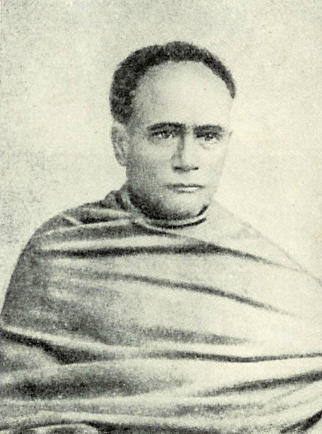
\includegraphics[width=0.75\marginparwidth]{./pictures/Ishwarchandra_Vidyasagar.jpg}}
    \caption{Ishwarchandra Vidyasagar}
    \vspace{0.8in}
    \framebox{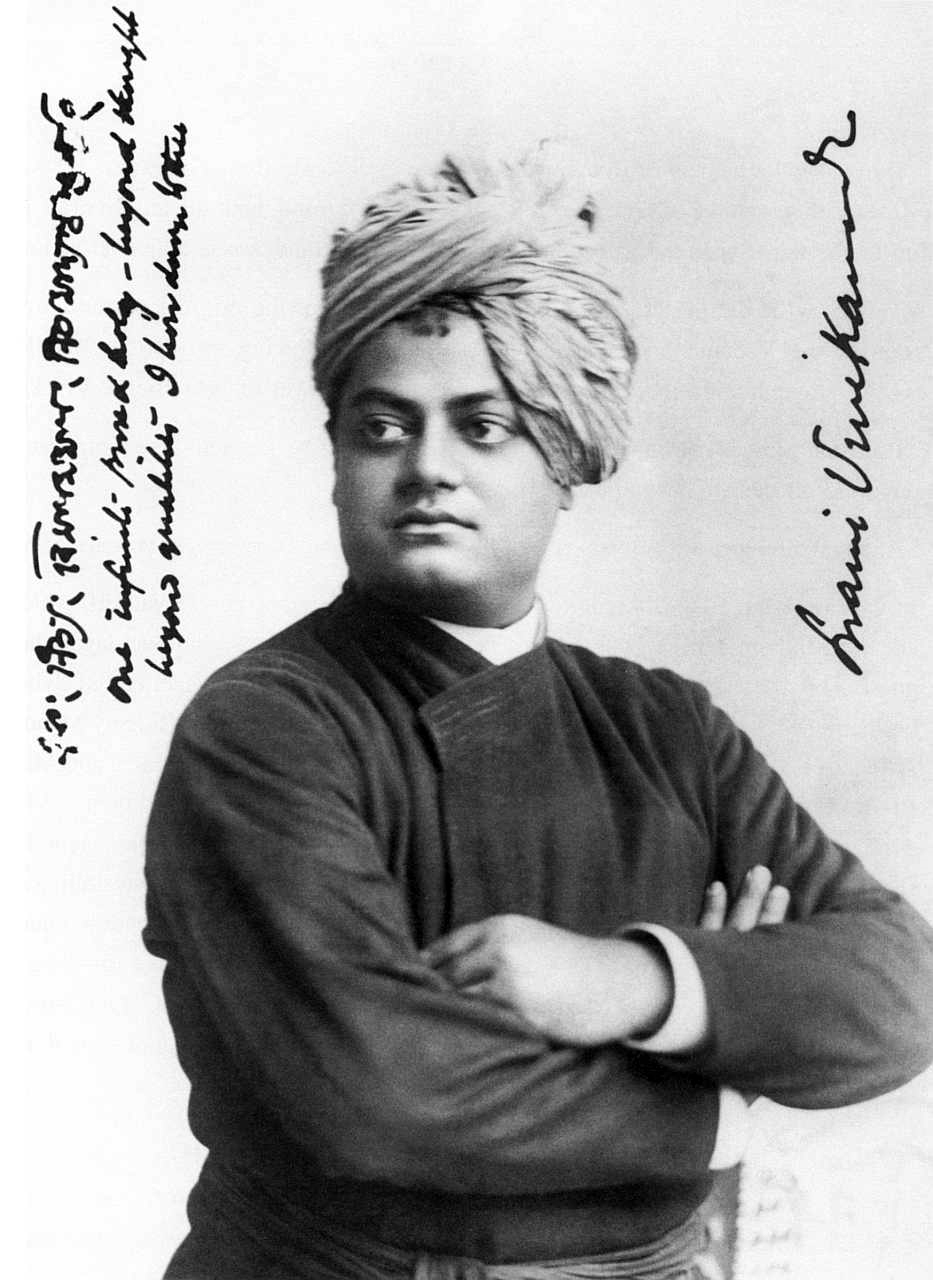
\includegraphics[width=0.75\marginparwidth]{./pictures/Swami_Vivekananda.jpg}}
    \caption{Swami Vivekananda}
    \vspace{0.8in}
    \framebox{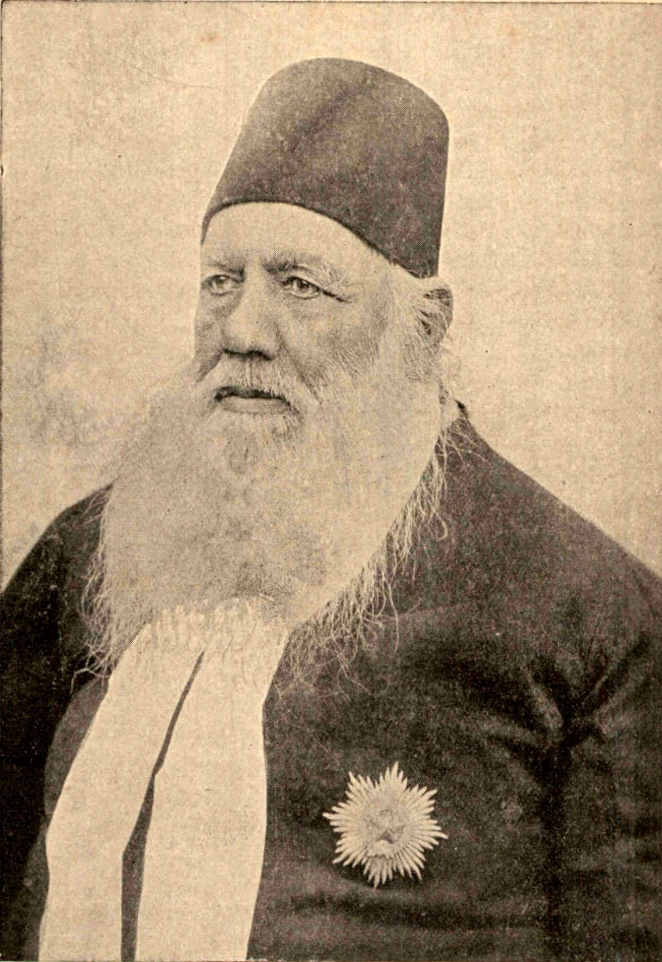
\includegraphics[width=0.75\marginparwidth]{./pictures/Syed_Ahmad_Khan.jpg}}
    \caption{Syed Ahmad Khan}
\end{marginfigure}

\section{An Economic Critique of Colonialism}
\begin{itemize}
    \item Dadhabai Naoroji, Justice Mahadev Govind Ranade and Romesh Chandra Dutt were the three early Moderates who solidified an economic critique of colonialism after they observed the failure of the Raj to bring about modernization in India
    \item They established the link between the economic regression of the subcontinent and the man-made colonial causes. This was not a natural or fated phenomenon
    \item They argued that Indian capital and not foreign capital would have to seed the industrialization of the nation, and this would be the pathto economic and social progress
    \item An increase in the volume of foreign trade in the 19th century was not a sign of progress because of the nature of the trade, which involved the export of raw material and the import of manufactured goods
    \item British economic policy was guided solely by the interests of the British capitalists, and not by any desire to nurture industry in India
    \item \Gls{drain theory}, once disseminated among the masses, got rid of the belief in the Raj providing good results and having good intentions for the Indian people. This shook the moral foundations of colonialism in the minds of the public
\end{itemize}

\section{The Fight to Secure Press Freedom}
\begin{itemize}
    \item Section 124A of the \gls{ipc} (the sedition law) restricted the freedom of the Press by criminalising the circulation of printed material that spread disaffection or discontent among the people
    \item Newspapers were the most effective means of political education, even among the illiterate masses who would listen to the material being read aloud
    \item Lokmanya Bal Gangadhar Tilak was the first prominent journalist to be prosecuted for sedition. His trial and imprisonment made him a well-known figure in the national consciousness
    \item Lokmanya Tilak's second trial for sedition and the six-year sentence in Burma to be served starting 1908 was to foreshadow Gandhiji being prosecuted under the same sedition laws in 1922
    \item Tilak plead not guilty to the charges of sedition, unlike Gandhi, reflecting the nascent nature of the Swarajya movement and the unwillingness to be openly defiant to the Raj
\end{itemize}

\begin{marginfigure}[-3.5in]
    \centering
    \framebox{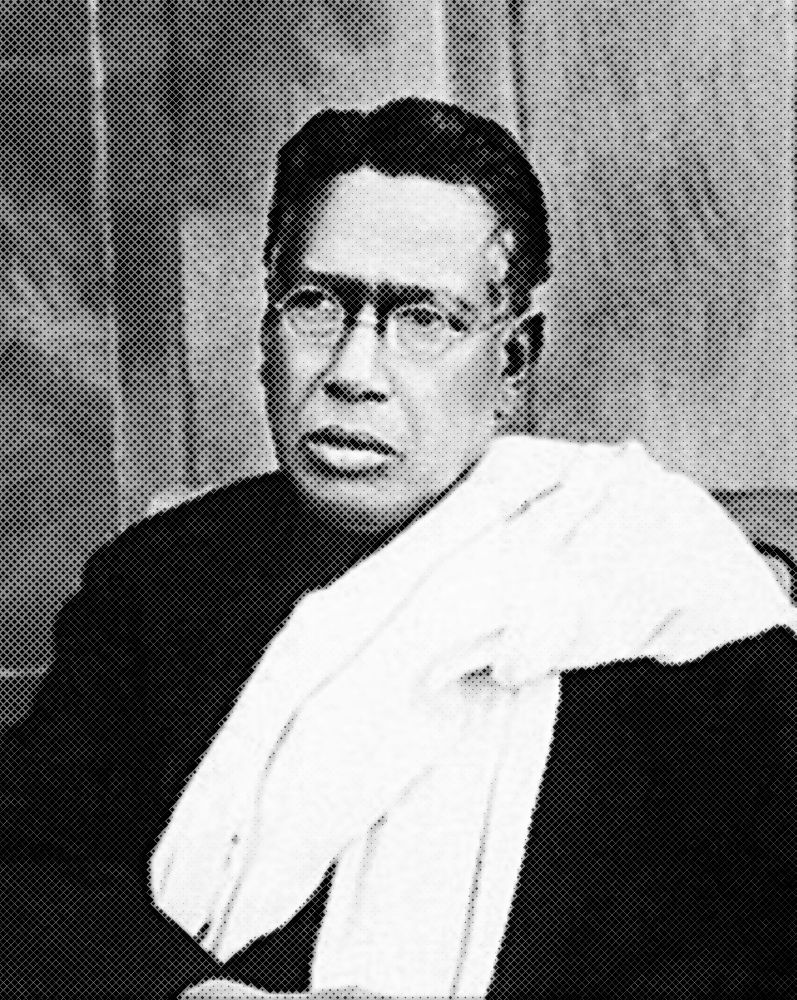
\includegraphics[width=0.75\marginparwidth]{./pictures/Bipin_Chandra_Pal.jpg}}
    \caption{Bipin Chandra Pal}
    \vspace{0.8in}
    \framebox{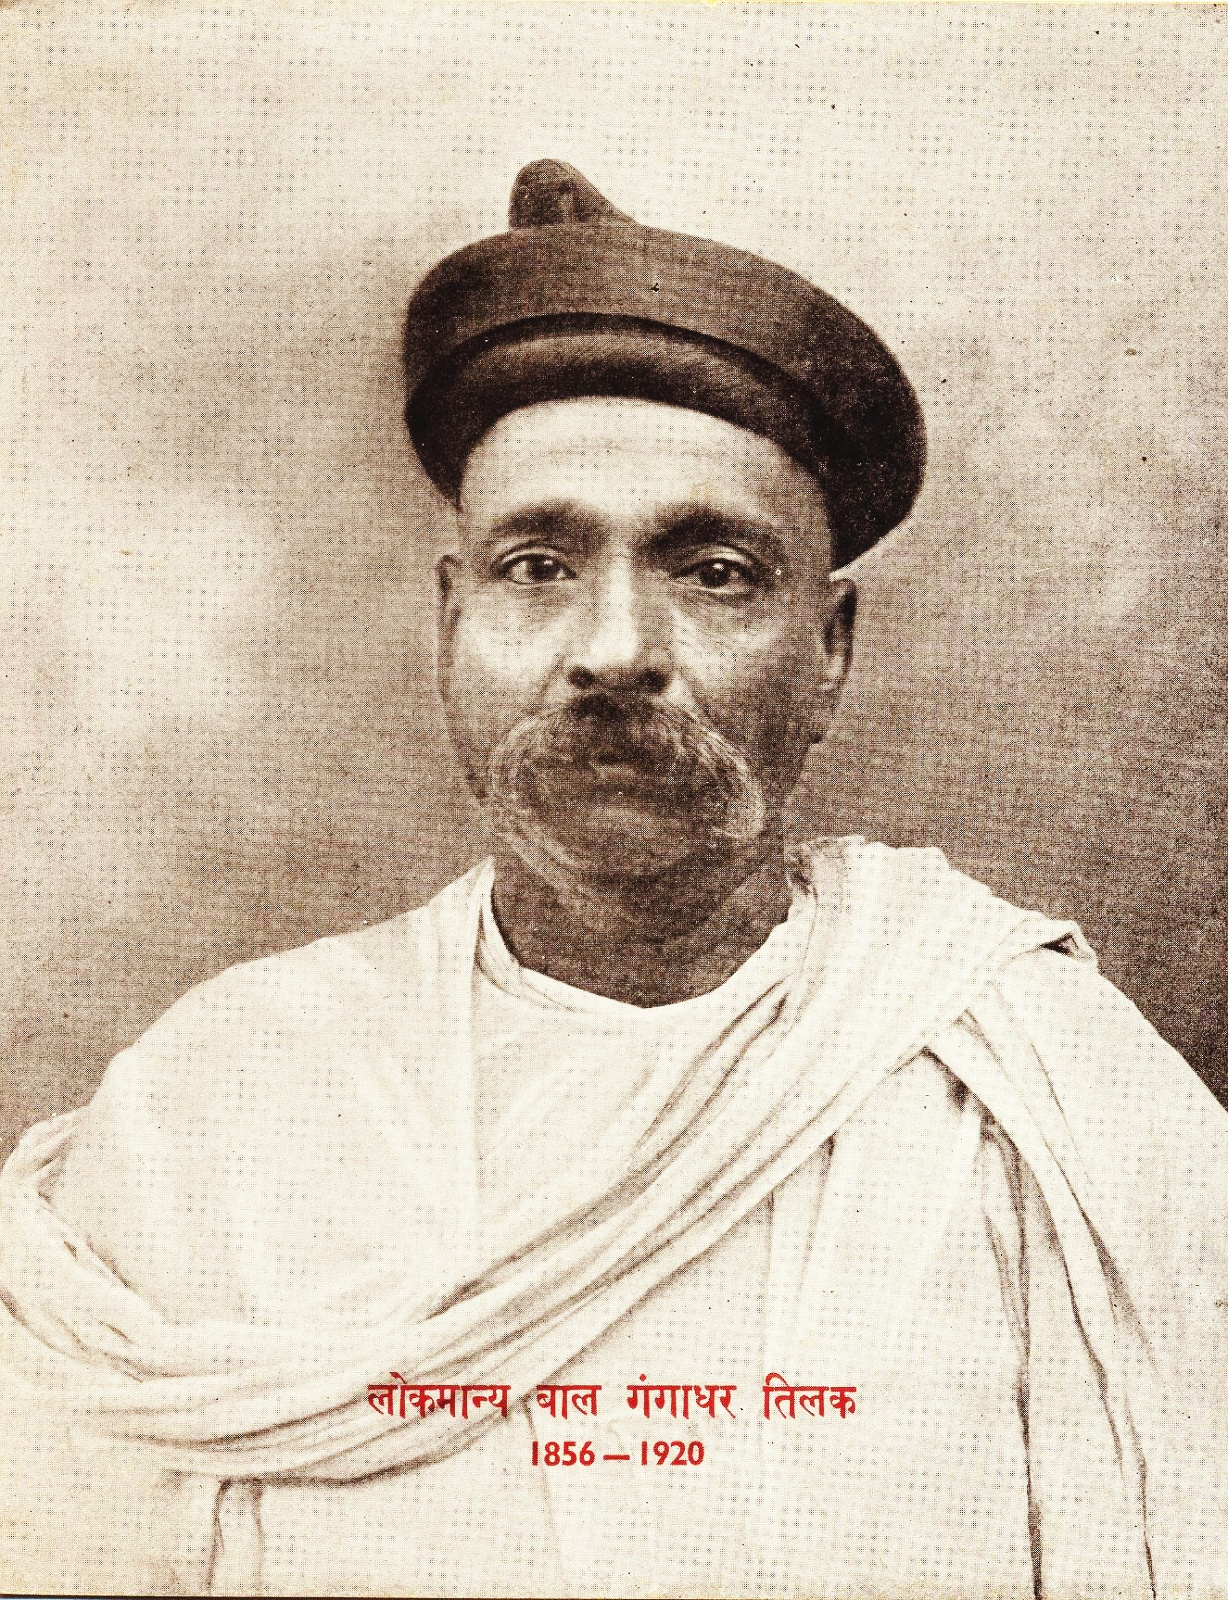
\includegraphics[width=0.75\marginparwidth]{./pictures/Lokmanya_Gangadhar_Tilak.jpg}}
    \caption{Bal Gangadhar Tilak}
    \vspace{0.8in}
    \framebox{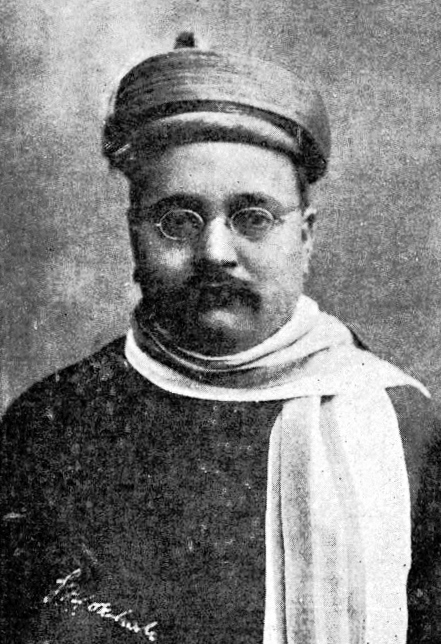
\includegraphics[width=0.75\marginparwidth]{./pictures/GK_Gokhale.jpg}}
    \caption{Gopal Krishna Gokhale}
\end{marginfigure}

\section{Propaganda in the Legislatures}
\begin{itemize}
    \item Imperial Legislative Councils were bodies with no real power meant to incorporate some Indian members so that the British could be made aware of Indian discontent in the aftermath of the 1857 revolt
    \item In practice, most Indian members appointed to the \glspl{ilc} were princelings, wealthy merchants or other stooges who towed the British line
    \item Demands for a model of self-government based on the colonies of Canada and Australia where the people elected their representatives into positions of economic and political decision-making began to gather steam in the 1900s
    \item G. K. Gokhale and Pherozeshah Mehta were the two most prominent members of the Legislative Councils who debated and critiqued legislation passed by the Raj and used their positions in the ILCs to further their statur as leaders of the freedom movement
\end{itemize}

\section{The Swadeshi Movement - 1903-1908}
\begin{itemize}
    \item Anti-parititon sentiment against the proposed partitioning of Bengal province into a Muslim-majority eastern portion and a Bengali-minority western portion sowed the seeds of the larger Swadeshi movement in 1900-1910
    \item In 1906, Dadhabai Naoroji took the important step of declaring formally that \Gls{swaraj} was the chief objective of the INC and the Swadeshi and Boycott movements had now grown larger than a mere anti-partition agitation
    \item Festivals, processions, meetings, and other new forms of mass mobilization and political education began to be used starting with the Swadeshi movement
    \item All India Muslim League was set up under the guidance of the Raj specifically to weaken the Swadeshi movement and introduce a communal obstacle to the efforts of the INC to unite all Indians under their banner
    \item Moderate forms of protest, such as petitioning and legal argument took a back seat during the Swadesh and Boycott movements, which were led by the extremist wing of the INC. The movements ended with the deportation or arrest of almost all of its leaders, and because it was impossible for mass mobilization to remain active for prolonged periods of time.
\end{itemize}

\section{The Split in the Congress and the Rise of Revolutionary Terrorism}

\begin{marginfigure}[-4in]
    \centering
    \framebox{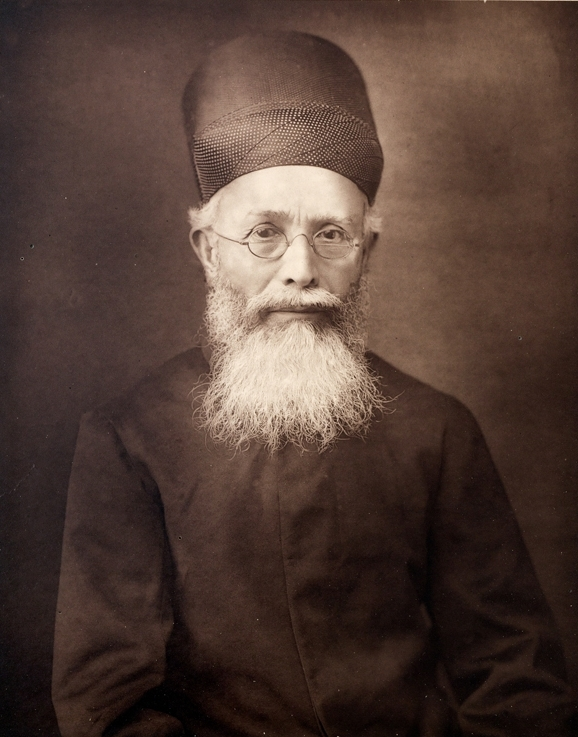
\includegraphics[width=0.75\marginparwidth]{./pictures/Dadabhai_Naoroji.jpg}}
    \caption{Dadabhai Naoroji}
    \vspace{0.8in}
    \framebox{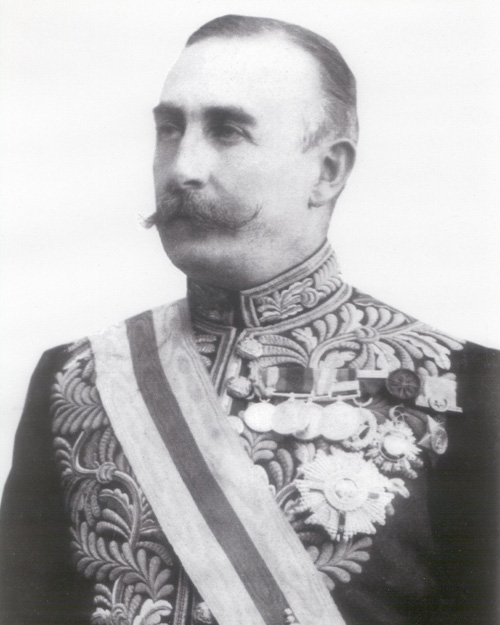
\includegraphics[width=0.75\marginparwidth]{./pictures/Viceroy_Minto.jpg}}
    \caption{Viceroy Lord Minto}
    \vspace{0.8in}
    \framebox{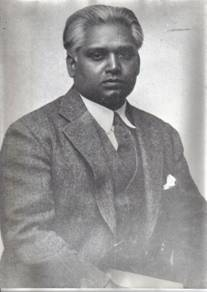
\includegraphics[width=0.75\marginparwidth]{./pictures/Tarak_Nath_Das.jpg}}
    \caption{Tarak Nath Das}
\end{marginfigure}

\begin{itemize}
    \item A policy of divide and rule was applied to the Extremist (led by Tilak) and Moderate (led by Gokhale) wings of the INC by then Viceroy Lord Minto once it became clear that it was not merely an academic body consisting of a few western-educated elite thinkers, but an organization capable of sustaining mass agitation as evidenced by the Swadeshi and Boycott movements
    \item Surat, 1907 was the Congress session that saw the resentment between the two wings of the party break out in violence with the police having to clear the premises. The Extremist wing's leadership either retired or emigrated or were exiled in the aftermath.
    \item Morley-Minto reforms included the introduction of Muslim constituencies to introduce a communal flavour to Indian political representation in the ILCs. Although the ILCs had more indirectly elected Indian members, they still lacked any real power
    \item 1908-1918 saw a period of revolutionary terrorism in Bengal which aimed to use violence and assassination of key officials as a means of 'protest by action'
\end{itemize}

\section{World War I and Indian Nationalism: The Ghadar}
\begin{itemize}
    \item jfadsfjhasdjk
\end{itemize}

\section{The Home Rule Movement and Its Fallout}
\begin{itemize}
    \item Lokmanya Tilak, after serving his ong sentence in Burma, planned to start the Home Rule League with Annie Beasant (who was working in Madras at the time) after failing to gain readmission into the Congress
    \item Tilak's Home Rule Leagues operated in Maharshtra, Karnataka and the surrounding regions, while Mrs. Beasant's Leagues were responsible for opeartion in the rest of the country
    \item Annie Beasant's arrest in 1917 led to the Home Rule movement gaining a popularity boost, with calls for civil disobedience and passive resistance starting to be heard
    \item The new Secretary of State Montague (who succeeded Lord Morley) sought to take a more pacifist stance with the Indians and instituted a policy of granting the Indians some kind of self-governance in the long run
\end{itemize}

\section{Gandhiji’s Early Career and Activism}
\begin{itemize}
    \item Gandhi's work in South Africa against the overtly racist apartheid regime was to last only a few months in 1893, but happened to stretch twenty years
    \item Having exhausted the `Moderate' methods of struggle, such as petitions, civil suits and other legal means by 1906, Gandhi then decided to turn to civil disobedience and Satyagraha
    \item By 1913, Gandhi had managed to get the Governor General of South Africa and the Viceroy of India to agree to most of his demands
    \item Gandhi's first political action was to emancipate the Indigo plantation workers in Champaran from their unfair contracts by debuting his methods of passive resistance and refusing the externemnt order imposed by the Raj
    \item Gandhi also arbitrated a wage hike dispute between mill owners and workers in Ahmedabad and as well as a land-revenue dispute in Kheda
    \item Protests against the Rowlatt Bills, meant to curtain freeomds in the name of maintaining order, inspired Gandhi to declare a nationwide Satyagraha, which would take the form of a non-violent strike
    \item Violence broke out in many parts on India however, and led tragically to the Jallianwala Bagh massacre in Amritsar
\end{itemize}

\section{The Non-Cooperation Movement - 1920-22}
\begin{itemize}
    \item Britain violating many of the promises it had made before the end of the First World War, and the toothless reforms they did bother propsing, led to a rapid rise in resentment and discontent among the Indians by mid 1920
    \item Non-cooperation was to include the boycott of government institutions, foreign goods, and striking,
    \item Violence against policemen in Chauri-Chaura, \gls{up} which led directly to Gandhi withdrawing the Non-Cooperation Movement in early 1922
    \item Gandhi withdrew the movement for other secondary reasons, incuding an ebb in the general nationalist vigour across the masses and concerns about the possibility of communalism creeping into the movement
\end{itemize}

\section{Peasant Movements and Nationalism in the 1920s}
\begin{itemize}
    \item Avadh in UP saw organized agricultural labour movements through the \textit{Kisan Sabha} and separately the \textit{Eka} struggles. Both of these movements were swiftly ended by the Raj through violent prosecution and repression
    \item In 1921, the Mappila Muslim teannts in the Malabar region rebelled against unfair land revenue policies.
    \item This rebellion only acquire a communal colour after the Raj began its violent repression along with its recruitment of local Hindu landowners to its cause against the Mappilas
    \item Bardoli, Gujarat was the site of the earlier satyagraha which Gandhi had canceled after the violence at Chauri Chaura, U.P.
    \item This was where the next big peasant movement began under the leadership of Vallabhbhai Patel in early 1928
    \item Eventually, the Raj was forced to revise its land revenue rates and concede to the demands of the Bardoli movement
\end{itemize}

\section{The Indian Working Class and the National Movement}
\begin{itemize}
    \item Collective bargaining and class action among the labour class in India had been deliberately ignored by the INC prior to the 1920s
    \item \gls{aituc} was the first national workers' body to be created in the 1920s
    \item Textile, railway and steelworking were the major industries at the time which employed the largest number of workers and thus contributed the most to union membership
    \item \gls{cpi}, which had seceded from the nationalist movement in the late 1920s, re-entered it in the 1930s
    \item Hitler's invasion of Russia let to the CPI withdrawing from the Quit India Movement of 1942, since the fatherland had to now be defended from the fascists Nazis
\end{itemize}

\section{The Struggles for Gurdwara Reform and Temple Entry}
\begin{itemize}
    \item Gurdwaras in Punjab were under the control of a priestly class until the 1920s, who were funnelling all of the temple revenue into their own pockets
    \item These priests were used very effectively by the Raj to subjugate the people of Punjab through their stranglehold on the religion
    \item \gls{sad} was founded in December 1920 to organize both the political struggle of the Sikhs as well as to manage the network of Gurdwaras that the reformers had successfully managed to liberate from the control of the priests
    \item By 1925, the Raj was forced to placate the Akali movement by conceding to the demands of its moderate wing and handing over complete control of all Sikh religious institutions to a body of elected Sikh leaders
    \item INC had chosen not to pursue social or religious reform till the 1920s, out of a fear of sowing divisions within the freedom movement
    \item It chose to reverse this position in 1923, and started a campaign to abolish untouchability, spearheaded by Gandhi
    \item Vaikom village in Travancore district, Kerala was the site of the first major satyagraha and harijan temple entry protest
    \item In 1936, the Maharaja of Travancore proclaimed entry into temples free for all people including harijans. Other provinces quickly followed suit, showing the amount of national attention this movement had garnered
\end{itemize}


\section{The Years of Stagnation - Swarajists, No-changers and Gandhiji}
\begin{itemize}
    \item Motilal Nehru and C.R. Das, split from the INC in 1928 to form the Swaraj Party, with their single issue being a cessation of boycotts and re-entering the election process to have their voices heard in the Legislative Councils
    \item This split howvever was not as emphatic as that of 1907, and compromises between the two camps were quickly reached out of a need to mantain a united front and a respect for Gandhi's decision being the final word in the matter
    \item Swarajists won a majority of the seats in the provincial and central Legislative Councils in the 1923 elections, either on their own or in coalition with local groups. Once inside, they voted out every piece of legislation put forth by the British, forcing them to be ratified by the Viceroy
    \item This became a major source of humiliation for the Raj and its illusion of having the goodwill of its subjects began to show cracks
    \item After a significantly wrose showing in the 1926 elections due to rising communalism and the compulsions of coalition politics, the Swaraj Party slowly ended its participation in the Legislative Councils by 1930
\end{itemize}

\section{Bhagat Singh, Surya Sen and the Revolutionary Terrorists}
\begin{itemize}
    \item Violent revolution in Northern India started with the \gls{hra} in 1924
    \item Bhagat Singh, Chandrashekhar Azad and Rajguru assassinated a police official in 1928 to avenge the killing of Lala Lajpat Rai in an earlier lathi charge incident
    \item They were tried and hanged in 1931, along with many of their fellow revolutionaries, in a series of highly publicized court trials
    \item Revolutionary activity was also organized on a large scale in Bengal province, by the \gls{ira}, especially in and around Chittagong
    \item By 1929, Bhagat Singh had abandoned his belief in violent revolution by the individual in favour of a Marxist mass movement as the most effective path to liberation
    \item Socialism, anti-communalism and atheism were the primary messages contained in Bhagat Singh and the revolutionaries' messaging to the masses
\end{itemize}

\section{The Gathering Storm 1927-1929}
\begin{itemize}
    \item Simon Commission was an all-white commission appointed in 1927 to look into the Indians' demands for further constitutional independence
    \item Boycotts and protests against the Simon commission (popularizing the ``Simon Go Back'' slogan) led to police repression that killed Lala Lajpat Rai in Lahore
    \item Lahore, 1929 was the INC session in which Jawaharlal Nehru, as the President, famously declared \textit{Purna Swaraj} as the only end goal of the Indian struggle against the Raj
    \item Gandhi regarded this session as the transfer or power and leadership from the older generation to the young, and insisted on appointing Nehru president over the objections of a majority of provincial Congress committees
    \item On Januray 26 1930, the Pledge of Independence was read all over the country to mark the start of the year of active protest
\end{itemize}

\section{Civil Disobedience 1930-1931}
\begin{itemize}
    \item On 6 April 1930, Gandhi inaugurated the Civil Disobedience Movement after marching to Dandi and picking up some salt from the beach in violation of the Salt tax laws
    \item Secondary forms of satyagraha called for non-payment of taxes and the boycott of foreign cloth and liquor
    \item On 25 January 1931, following a Round Table Conference in London attended by Indian representatives to discuss the constitutional future of India, Gandhi was released from jail
    \item Negotiations between the Viceroy Lord Irwin and Gandhi led to a truce in March 1931 called the Gandhi-Irwin pact
    \item Although the pact is seen as capitulation by Gandhi to bourgeoisie interests or as a betrayal, it can be understood as a recognition of the satyagraha losing steam and a timely extraction of as many concessions as possible from the Raj
\end{itemize}

\section{From Karachi to Wardha: The Years from 1932-1934}
\begin{itemize}
    \item In March 1931, the INC passed the Karahi resolution which was to constitute the essence of the constitution of independent India and guide Congress policy in later decades
    \item After signing the Gandhi-Irwin pact, the British government decided to reverse their policy of negotiating with the INC on equal terms and went back on their earlier promises
    \item In the years 1931-1934, the Raj crushed all attempts at mass organization, censored any reporting by the press on the freedom movement, and established Civil Martial Law
    \item Gandhi undertook an extensive travel campaign and multiple fasts to put an end to untouchability and liberate the untouchable castes, whom he called \Glspl{harijan}
    \item This movement was not to intersect with Ambedkar's demands for the abolition of the caste system itself. Tackling inter-marriage and inter-dining among the castes was not in Gandhi's interests during this time
\end{itemize}

\section{The Rise of the Left-Wing}
\begin{itemize}
    \item Socialism and Marxist ideology acquired a foothold in Indian politics in the 1920s and 1930s through the formation of the CPI, the \gls{csp} and in the rise to prominence of Nehru within the INC
    \item Nehru, while criticizing Gandhi in 1933 for his belief in the harmony between classes and rejection of the Marxist class perspective, also defended his contribution to the freedom movement in raising the political consciousness of the masses
    \item After the Congress of the Communist International session 1935 held in Moscow, the Communists were to cooperate with other socialist and anti-imperialist forces to face the coming thresat of fascism
    \item This led to the CPI, which had alienated itself from the mainstream of the freedom movement by splitting from the INC, reintergrating itself into the main party
    \item The CSP was founded jointly by Jayaprakash Narayan and associates in 1934 with the objective of working under the INC umberella with the aim of steering it leftward and compelling it to adopt a socialist program
\end{itemize}

\section{The Strategic Debate 1934-1937}
\begin{itemize}
    \item Nehru wished to take up the socialist path forward in the lull following the end of the Non-cooperation movement in 1934.
    \item Existing camps wanted to either follow Gandhi in reconstructive work in the villages or the Swarajists in participating in the Legislative Assemblies and contensting elections
    \item British strategy involved follinwg up the open repression with a phase of reforms and eyewash legislation designed to wean the moderate and constitutionalist section of the INC away from the mainstream freedom movement
    \item In 1935, the Government of India Act was designed to create a shambolic provincial body that was supposedly autonomous and had legislative powers. In truth, the governors and viceroy still had direct control over sensitive subjects and exercised extensive veto powers behind the scenes
    \item In 1937, elections to the ILC and the Provoncial Legislative Assemblies were contested by the Congress with an agenda wholly rejecting the 1935 Act, and the broad themes of the freedom movement
    \item Their performance in the elections helped Nehru come to terms with the fallacy of an uninterrupted struggle and see the light in Gandhi's ebb and flow strategy of non-cooperation
\end{itemize}

\section{Twenty-eight Months of Congress Rule}
\begin{itemize}
    \item In the provinces where it assumed office, the Congress immediately set about repealing curbs on press freedom, releasing political prisoners, restoring whatever civil liberties they could
    \item Attempts to reform the land revenue system and abolish the zamindari practice were hampered by the limits placed on the INC's powers by the Governors and the viceroy
    \item Also the multi-class nature of the freedom movement meant that the INC could not wholly antagonize the landlord class in its attempts to make reparations for the peasant classes
    \item INC Ministries promoted tenancy reform, pro-labour reforms targeting the industrial sector, and social reforms aimed at Harijan upliftment
    \item Left wing groups within the INC were dissatisfied with its handling of extra-legal protests and its dilemma in nurturing the freedom movement while also being the government in power
    \item Breaking one of the other myths propping up the Raj, that Indians were not fit to rule themselves, was the major accomplishment of the Ministries
\end{itemize}

\section{Peasant Movements in the 1930s and '40s}
\begin{itemize}
    \item Pressure from the Great Depression starting in 1929 and the Non-cooperation movement in the 1930s led to mass organization among the peasants starting with the formation of the \gls{aiksc} in 1936 at Lucknow
    \item Agrarian legislation, motivated by the first Kisan Manifesto of 1937, was pushed for by the Congress Ministries during their 28 month term in power
    \item Anti-war sentiments held by the Kisan Sabhas and other Socialist sections of the Congress attracted severe repression from the Raj with the onset of World War II
    \item Major leaders left the Kisan Sahbha Congress because of the pro-War anti-fascist party line enforced by the Commnunist flank
    \item In 1945, the end of WWII meant the resumption of the struggle to abolish zamindari, which found success post-independence in Bengal and Punjab
\end{itemize}

\section{The Freedom Struggle in Princely India}
\begin{itemize}
    \item \Glspl{praja mandal} began to form in many princeoly states in the aftermatch of the Non-Cooperation movement of 1920
    \item By 1939, the Government of India Act and the 28 month tenure of the Congres Ministries in British India accelerated political mobilization and awareness among the people of the princely states
    \item In 1939, the \gls{aispc} elected Nehru their president, formally merging the two organizations and tearing down the barrier that the INC had previously maintained between the freedom movements in British and princely India
    \item For 30 years, the princely state of Rajkot was ruled by Lakhajiraj, a progressive monarch who placed great value in the development of industry, and established a legislative body full of elected representatives of the people
    \item His successor, Dharmendra Singhji, was the polar opposite and indulged in hedonism to the point of squandering away
    \item Satyagraha punctuated by brief but unsuccessful negotiatoins with the British resident in Rajkot, along with the Dewan, who was the real center of royal power, culminated in Gandhi arriving in Rajkot and beginning a fast unto death in March 1939
    \item In Hyderabad, the \Gls{nizam} sought to impose Islam and Urdu in an otherwise majority Hindu state, along with repressing any efforts to promote the other languages of the realm (Marathi, Kannada and Telugu)
    \item Although the State Congress (a body unrelated to the INC but receiving its support) withdrew its agitations for fear of being subsumed by the communal agitations of the \Gls{arya samaj} in the late 1930s, the Quit India movement of 1942 brought together formally the subjects of the Raj and the princely states in their demand for a free India
    \item After Viceory Mountbatten announced 15th August 1947 as the date the Raj would hand over power to the Indians and would no longer have dominon over the princely states, the Nizam decided to refuse accession to the union
    \item From 7th August 1947, the Nizam used armed paramitary forces to repress the protestors and quell strikes. On 18th September 1948, when the Indian Union moved its army into Hyderabad, the Nizam finally surrendered and acceded to the Union
    \item Unlike Hyderabad, the rulers of most other states realized the extent to which they were propped up by the British government in spite of its claims of non-interference. This led to them readily signing the Instruments of Accession once the British left India
\end{itemize}

\section{Indian Capitalists and the National Movement}
\begin{itemize}
    \item Capitalists under the Raj grew in spite of colonialism, not because of it, as is often the case in other colonies. They insisted on the use of independent capital, import substitution strategies and a refusal to be subservient to the Raj.
    \item In 1927, the \gls{ficci} was the first all-India lobbying organization founded by the capitalist class to agitate for its interests
    \item Non-constitutional forms of struggle, such as satyagraha were regarded with skepticism by the capitalists for fear that they would attract a social revolution, and treaten the idea of capitalism itself
    \item While capitalists did donate to the INC, these funds were far from the primary means of sustenance for the party and the freedom movement. Such contributions did not lead to sny influencing of INC policy or softening of their anti-imperialist stance
\end{itemize}

\section{The Development of a Nationalist Foreign Policy}
\begin{itemize}
    \item In the 1870s and 1880s, the Indian army was used to wage wars in Afghanistan and Egypt to further the imperial interests of Britain, at the expense of Indian wealth and manpower
    \item Leaders of the Indian freedom movement expressed their sympathy and support for anti-imperialist struggle in many countries in Asia and Africa from the 1870s to the 1940s
    \item Fascism prevailing in Japan, Germany and Italy in 1936 led the INC to establish a Foreign Relations department and to speak out on the international stage against fascist actions undertaken by each of these nations
    \item Nehru's visit to Soviet Russia in 1927 greatly influenced his ideology in a Marxist and socialist direction. He admired Soviet Russia as the single biggest force against imperialism and fascism in the world, in spite of his revulsion to Lenin's purges of the 1930s
\end{itemize}

\section{The Rise and Growth of Communalism}
\begin{itemize}
    \item Communalism rests on the foundation that the political, social and economic interests of a people are based only on their religious identity and that the interests of one such religious group can never be aligned with another
    \item It also claims that all political leaders are religious leaders either openy or behind a mask
    \item Finally, communalism asserts that different religious groups have to have hostile intersts and be antagonistic to each other as a matter of dogma
    \item At the time, Indians were united primarily along linguistic, cultural and class lines than religious lines. Claiming the exact opposite was one of the basic assumptions of communalism
    \item Communalism was not a holdover from anceint or medieval Indian politics, which ignored the masses wholly. Mass mobilization and participation had to be invented as a form of political action (as happened post 1857 in India) for socialism, nationalism and communalism to emerge as ideologies
    \item Communalism first took hold among the urban middle class and rural youth who received education and no longer had the ability or interest in the old agricultural livelihoods. Communal reservations in service sector jobs under the Raj were a myopic but effective argument in favor of communalism
    \item Since religious grouping in India tended to coincide with class and social grouping, communalists could misattribute tension between the classes or between social groups as a communal dispute, even though there was no underlying communal cause of the conflict
    \item Divide and Rule policies emplyed by the Raj failed on all counts by the 1920s except their efforts to use communalism to sow division within the national movement, especially by offering the defence of religious minorities from the majority Hindus as a justification for British colonial rule
    \item Deliberate failure by the Raj to curtail communalist propaganda, rioting, and pandering to the demands of minority communal leaders were all contributing factors to the growth of communalism during the national freedom movement
    \item Distorted teachings of history formally at the school and informally through popluar written and spoken word, presented Indian history as the story of a once mightly Hindu culture that fell into a permanent Dark Age under the `foreign' rule of Muslim emperors. These false interpretations were encouraged by British historians and quickly latched onto by communal propagandists
\end{itemize}


\section{Communalism — The Liberal Phase}
\begin{itemize}
    \item Syed Ahmed in 1887 started communal attempts to oppose the nascent National freedom movement because of his belief in placating the Raj and the wealthy landowners as the path to Muslim upliftment and prosperity
    \item Tyranny of the Hindu majority if they were to overthrow British rule, a permanent incompatibiltiy and hostility of Hindu and Muslim political interests, religious reservations in government jobs, education and electoral seats were the primary elements of his propaganda
    \item After the Swadeshi movement of 1905-06, a large section of Muslim intelligentsia abandoned their policy of political inaction and joined the INC
    \item All India Muslim League was founded in 1907 as a loyalist, conservative, communal organization by some elite Muslims and monarchs
    \item Anti cow-slaughter, anti-Urdu pro-Hindi, and accusing the INC of sacrificing Hindu interests to appease Muslims were the founding tenets of Hindu communalism in the late 1890s
    \item Separate electorates for minoritties where only one religion could vote and run for seats came with the Morley-Minto reforms of 1907. These were used as a potent justification by communalists to preach cooperation with the Raj and abstaining from the INC and the freedom movement
    \item From 1912 to 1924, the Muslim League came to be dominated by a more nationalist ideology, which aligned more closely with INC positions against imperialism, but wasn't secular. It believed in opposing the Raj out of a desire to move towards a global \Gls{caliphate}, not out of any allegiance towards India as a nation
    \item Khilafat activists largely harmonized with the INC after the Lucknow Pact signed by Tilak and Jinnah in 1916. They did however insist on looking at political questions with a religious lens, and put Muslim solidarity over and above Indian identity, thus keeping the embers of communalism alive
    \item In 1923, after the Non-cooperation movement had been withdrawn, the Hindu Mahasabha and a resurgent communal Muslim League began to rise to prominence. Several INC leaders were forced by the communal pressure to compromise with the demands of these communal groups
    \item Instead of opposing communalism at the grassroots, the INC chose a top-down approach. They held negotiations with communalist leaders in an attempt to better merge them into the Freedom movement, and thus implicitly legitimized their status as the representatives of the respective religious groups
    \item This strategy was largely a failure and the repeated movement of the communal ideology toward the extreme meant that moderate leaders within those communalist groups were forced to keep moving to the fringe or lose their positions of power (M. A. Jinnah within the Muslim League being the most famous example)
\end{itemize}

\section{Jinnah, Golwalkar and Extreme Communalism}
\begin{itemize}
    \item It was only after 1937, when communalism moved into its more extremist, fascist phase, that it gained a broad base of appeal. The landlords and wealthy began to shift towards communalism to get the masses within their religion to defend their class interests
    \item M.A. Jinnah's life illustrates the slippery slope of communalism very well. He started off as a liberal communalist, crowned the 'Ambassador of Hindu-Muslim Unity' when he bitterly opposed the Muslim League's formation in 1906
    \item In response to Gandhi's plan to commit civil disobedience in 1920, Jinnah left the INC and turned to liberal communalism. He joined the Muslim League and became a proponent of working within the law and using litigation to wrest some power within the British Imperial system
    \item After a poor showing in the 1937 elections running a nationalist INC adjacent manifesto with the Muslim League, Jinnah saw the reality of the Raj having already fulfilled all of the demands made by liberal communalism and felt compelled to slide into extreme communalism
    \item By 1939, leaders of the Hindu Mahasabha (V.D. Savarkar) and \gls{rss} (M.S. Golwalkar) were establishing the primary message of Hinduism under threat from Islam and the need for a Hindu nation succeeding the Raj
    \item Minority communities had to either glorify and accept Hinduism or resign themselves to a second-class existence in India, or better yet be ejected from the country if they chose to practice their religion
    \item In 1937, Jinnah wanted the INC to declare itself a Hindu body and give up its claims of being a secular organization representing all Indians - a non starter for the INC. By 1940, the only card left to Jinnah was to put forth the demand for a separate homeland for the Muslims - Pakistan.
\end{itemize}

\section{The Crisis at Tripuri to the Cripps Mission}
\begin{itemize}
    \item Subhash Chandra Bose in 1939, decided to turn the INC's policy direction away from the supposed rightists' path of conciliation with the Raj and towards a more violent, extremist path
    \item After being driven to resign from the position of president by Gandhji and his faction in the Congress working committees at the Tripuri session of the INC, Bose formed the Forward Bloc within the Congress in March 1939
    \item British hostility to the idea of granting India a path to Swaraj after the war and only paying lip service to the idea of consulting with INC representatives in this regard expedited the need for another active Satyagraha movement
    \item A lack of Hindu-Muslim unity, endemic corruption within the INC after 1938-39, and the fact that all possible negotiations had not been exhausted, led the leadership to call off demands for an immediate civil disobedience movement
    \item By May 1941, thousands of individual satyagrahis had been convicted by the Raj after they performed individual acts of civil disobedience in accordance with Gandhi's plan of warming up the masses with a small scale satyagraha
    \item Under pressure from his parliament, Churchill was forced to send Stafford Cripps to India in 1942, with a proposal to grant India dominion status after the war in exchange for its active participattion in the war effort aganst the Axis powers
\end{itemize}

\section{The Quit India Movement and the INA}
\begin{itemize}
    \item Instability in the Raj because of the war effort, reports of the British abandoning their subjects in south-east Asia when faced with the might of the Japanese, and a need to rouse the masses in preparation for a possible invasion of India by Japan were the main reasons the Quit India movement was initiated in August 1942
    \item Severe repression by the military and sweeping arrests of the top INC leadership followed in the weeks after the movement was launced
    \item Gandhi decided to enter a 21 day fast while in prison which had the effect of greatly raising morale among the masses because of the Raj remaining obstinate in its refusal to accommodate Gandhi's demands or to release him
    \item Successful attempts were made to set up parallel governments in Ballia, U.P., Satara and Tamluk, Bengal by destroying British logistics and forcing the officials to hand power over to the local resistance. These governments only lasted a few weeks till the military came marching in to wrest control back using their superior might
    \item This movement was significantly more spontaneous and less organized in a top-down fashion than the 1920, 1930-31 or 1932 movements because of steps taken by the INC to make the masses politically aware of their programme and instill in them the basic forms that Satyagraha should take, even in the absence of a central leadership
    \item By June 1945, the leadership of the INC had been released on health grounds or otherwise to participate in the British offer for partial transfer of power in the Shimla Conference, marking the end of the movement
    \item In September 1942, the first \gls{ina} division was formed in Malaya by former soldiers in the British Indian Army, with an aim to cooperate with the Japanese in their anti-British efforts, and to prevent a potential invasion of India by the Japanese
    \item While accompanying the Japanese in their invasion of Imphal, the INA were forced to endure racism and inferior treatment by the Japanese forces, eventually breaking their morale and preventing them from achieving any military victories against the Raj
\end{itemize}

\section{Post-War National Upsurge}
\begin{itemize}
    \item Repression in the aftermath of WWII had only made the masses more determined in their anti-British stance, and the INC leadership found no signs of fatigue or demoralization when they were released in June 1945
    \item INC (and the Muslim League in Muslim reserved constituencies) swept the elections in 1945 campaigning on the issues of holding the Raj officials to account for their repression in 1942, as well as the defence of the captured INA troops
    \item These trials mobilized groups hitherto loyal to the Raj, such as Indian soldiers, government officials and landowners, alarming the British Intelligence Service and leading to great leniency by the Government in their releasing of the men on trial
    \item Armed forces personnel in many provinces revolted violently and were joined by strikes and hartals by the masses in the city in response to the INA trials. Such insubordination had an extraordinary effect on British morale
    \item Protests were led by the CSP, CPI and Forward Bloc, with no direct Congress participation or authority. Individual INC leaders did participate in some of the protests outside of their role in the Congress
    \item Since the INC has a strict policy of peaceful negotiation first and civil disobedience after, the INC leaders implored the violent mutineers and protesters to abandon their struggle and go home, to lay the ground for negotiating with the 1946 Cabinet Mission called for by Prime Minister Clement Attlee
\end{itemize}

\section{Freedom and Partition}
\begin{itemize}
    \item Raj hegemony oer the Indian people depended on the aura of invincibility, the belief in their best intentions for the masses, and the myth that Indians were incapable of governing themselves
    \item Indian Civil Service, which provided the backbone of Britihs beaureaucracy in India, was crumbling starting in 1919, with a decreasing white representaion within the service and a lack of promising fresh graduates willing to join the service from Britain with the start of WWII
    \item INC Ministries formed in th 1937 elections turned the tide in the belief held by loyalists and servicemen as to the efficacy of the Raj's dual policy of conciliation and repression. It also made real the possibility that the servicemen might have to serve the same INC that they helped repress after India gained independence
    \item After reaching the conclusion that they would have to quit India by early 1946, the Raj decided to enter negotiations with the INC with an initial stance against any partition of the country in the interest of leaving India a significicant military and trading ally
    \item Attlee in February 1947 fixed the date of withdrawal as 30 June 1948, with the caveat that power would be transferred to multiple centers if the existing provisional government was not fully representative of the nation's minorities
    \item This pushed Jinnah into threaening communal violence and completely abandoning all participation in the interim government in his attempts to secure Pakistan
    \item Lord Mountbatter, the last Viceroy of India, took charge in early 1947, with the modified strategy of granting Jinnah his sovereign state, but compensating the INC by fulfililng all of their remaaining demands
    \item From 3 June to 15 August 1947, hasty and haphazard divisions of the assets of British India and the land boundaries between India and Pakistan had to be drawn up in preparation for Independence Day. This moving forward of the British withdrawal is considered a major reason for the violence surrounding partition
    \item Communal violence and the loosening of its grip on the administration of Muslim-majority provinces led the INC leaders to agree to the Mountbatten plan and give in to Jinnah's demands for a sovereign Muslim nation
    \item Secondary reasons for the INC conceding the demand for partition included their delusions of Partition being temporary, peaceful and reversible, if the masses were given the benefit of hindsight
\end{itemize}

\section{The Long-Term Strategy of The National Movement}
\begin{itemize}
    \item Two ideas underpinning the British government's hegemony over the Indian people were the belief in their benevolt commitement to 'modernizing' India and in their military might being so absolute that any opposition to them was futile
    \item Nationalist leaders sought to develop a counter-hegemonic movement which eroded these two pillars of British hegemony, by raising the political consciousness of the masses, increasing the political space available to them under the Raj and to weaken the hold of the Raj over its civil and military services, manned by a moajority of Indians
    \item Since the masses could only participate in civil disobedience for a limited time, until government repression burnt through their reserves of patience and wealth, the national movement had to alternate between phases of extra-legal satyagraha and legal constitutional action
    \item Gandhi devised a constructive work programme to keep the masses politically conscious during the passive phases of the freedom movement, pursuing his goals of Harijan upliftment, Hindu-Muslim unity, boycott of foreign goods, and the struggle against untouchability
    \item Mass movements, by their very nature would have been unsustainable if they hadn't been non-violent, enabling even the common peasant, and women to participate in great numbers. They also flummoxed the colonial authorities by exposing their evil nature when they inevitably chose violent repression as a means to deal with non-violent civil disobedience
\end{itemize}

\section{The Indian National Movement — The Ideological Dimension}
\begin{itemize}
    \item Using India as a market for British manufacturing, thus destroying Indian handicrafts, and draining India's wealth to Britain were the two main economic arguments against colonialism as delivered to the Indian masses from the 1890s to 1920s
    \item INC policy included civil liberty, representative democracy based on universal adult franchise, secularism, minority rights, state ownership of key large-scale industries
    \item Pro-poor policy to be implemented by a central welfare state, guaranteeing education, fair land revenue policies and the protection of workers' right were the chief pillars of the INC economic policy
    \item Although Gandhi did not agree with Nehru's socialist ideas and imitation of the Soviet Five-Year Plans, he was still in agreement about state ownership of large industries and nationalization of all key manufacturing and service sector industries
    \item INC policy was not very clear-cut when it came to the abolition of caste and women's rights. This tragically led to the lack of clear policymaking in Independent India aimed at addressing these social issues
\end{itemize}